%! Author = mac
%! Date = 2022/4/21

% Preamble
\documentclass[UTF8]{ctexart}
\usepackage{geometry}
\geometry{left = 1.0cm, right = 1.0cm, top = 2.0cm, bottom = 1.0cm}
\usepackage{graphicx}
\usepackage{amssymb}
\usepackage{amsmath}
\usepackage{textcomp}


% Document
\begin{document}
\section*{气体训练2}
\paragraph{高考中的变质量}
\kaishu{}
\paragraph{}
    1.(2020高考)为方便抽取密封药瓶里的药液,护士一般先用注射器注入少量气体到药瓶里后再抽取药液,
如图所示,某种药瓶的容积为0.9mL,内装有0.5mL的药液,瓶内气体压强为$1.0 \times 10^{5}Pa$,
护士把注射器内横截面积为$0.3cm^{2}$、长度为0.4cm、压强为$1.0 \times 10^{5}Pa$的气体注入药瓶,
若瓶内外温度相同且保持不变,气体视为理想气体,求此时药瓶内气体的压强。

\begin{figure}[htbp]
% \centering
\paragraph{} 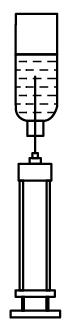
\includegraphics[height = 5.0cm]{/Users/mac/Desktop/ALLDATA/程序/TEX/实验一/图片1}\label{fig:figure}
\end{figure}
解:
瓶内气体体积$V_{0} = (0.9-0.5) \times 10^{-6} m^{3} = 4 \times 10^{-7}$

因为瓶内气体压强也为$p_{0}$,考虑瓶内与瓶外气体总体积为$V_{s} = V_{0} + V_{a} = 5.2 \times 10^{-7} m^{3}$

瓶外气体注射后,瓶内气体体积不变,发生等温变化:

\begin{gather*}
    p_{0}  V_{s} = p_{1}  V_{0}\\
    p_{1} = \frac{p_{0}V_{s}}{V_{0}} = 1.3 \times 10^{5}Pa\\
\end{gather*}


\paragraph{}
    2.(2020高考)甲、乙两个储气罐储存有同种气体(可视为理想气体)。甲罐的容积为V,罐中气体的压强为p;乙罐的容积为2V,罐中气体的压强为$\frac{p}{2}$。
    现通过连接两罐的细管把甲罐中的部分气体调配到乙罐中去,两罐中气体温度相同且在调配过程中保持不变,调配后两罐中气体的压强相等。
    求调配后:

    (1)两罐中气体的压强

    (2)甲罐中气体的质量与甲罐中原有气体的质量之比

解:
(1)可以认为乙罐气体先发生等温变化再发生等压变化,等压变化时压强变为p,即:
\begin{gather*}
    2V \cdot \frac{p}{2} = V_{1} \cdot p\\
    V_{1} = V\\
\end{gather*}
随后所有气体共同发生等压变化:
\begin{gather*}
    (V_{1} + V) \cdot p = 3V \cdot p_{1}\\
    p_{1} = \frac{(V_{1} + V) \cdot p}{3V} = \frac{2}{3}  p\\
\end{gather*}

(2)同一压强同一温度下气体体积比等于质量比,可列:
\begin{gather*}
    p \cdot V = \frac{2}{3}p \cdot V_{2}\\
    \frac{m_{2}}{m_{0}} = \frac{V}{V_{2}}\\
\end{gather*}
整理得:
\begin{gather*}
    V_{2} = \frac{3}{2}V\\
    \frac{m_{2}}{m_{0}} = \frac{2}{3}\\
\end{gather*}

\paragraph{}


    3.(2020高考)潜水钟是一种水下救生设备,它是一个底部开口、上部封闭的容器,外形与钟相似。
    潜水钟在水下时其内部上方空间里存有空气,以满足潜水员水下避险的需要。
    为计算方便,将潜水钟简化为截面积为S、高度为h、开口向下的圆筒;工作母船将潜水钟由水面上方开口向下吊放至深度为H的水下,如图所示。
    已知水的密度为$\rho$,重力加速度大小为g,大气压强为$p_{0}$,$H \gg h$,忽略温度的变化和水密度随深度的变化。

    (1)求进入圆筒内水的高度l

    (2)保持H不变,压入空气使筒内水全部排出,求压入的空气在其压强为$p_{0}$时的体积。

\begin{figure}[htbp]
% \centering
\paragraph{} 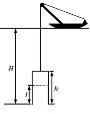
\includegraphics[height = 3.0cm]{/Users/mac/Desktop/ALLDATA/程序/TEX/实验一/图片3}\label{fig:figure1}
\end{figure}

 解:
(1)由题可列:
\begin{gather*}
    p_{0} + \rho gH = \rho gl + p_{1}\\
    p_{0}Sh = p_{1}S(h-l)\\
\end{gather*}
整理得:
\begin{gather*}
    p_{0} + \rho g(H-l) = p_{1}\\
    l = h - \frac{p_{0}h}{p_{1}}\\
\end{gather*}
又$H \gg h \textgreater l$,则
\begin{gather*}
    p_{1} = p_{0} + \rho gH\\
    l = \frac{\rho gHh}{p_{0} + \rho gH}\\
\end{gather*}

(2)由题知钟内空气在压强为$p_{0}$时的体积$V = Sh$:
\begin{gather*}
    p_{0}(V_{2} + V) = p_{2}V\\
    p_{2} = p_{0} + \rho gH\\
\end{gather*}
即:
\begin{gather*}
    V_{2} = \frac{p_{2} - p_{0}}{p_{0}} V = \frac{\rho gHSh}{p_{0}}\\
\end{gather*}

\paragraph{}


\paragraph{}
    4.(2020高考)中医拔罐的物理原理是利用玻璃罐内外的气压差使罐吸附在人体穴位上,进而治疗某些疾病。
    常见拔罐有两种,如图所示,左侧为火罐,下端开口;右侧为抽气拔罐,下端开口,上端留有抽气阀门。
    使用火罐时,先加热罐中气体,然后迅速按到皮肤上,自然降温后火罐内部气压低于外部大气压,使火罐紧紧吸附在皮肤上。
    抽气拔罐是先把罐体按在皮肤上,再通过抽气降低罐内气体压强。
    某次使用火罐时,罐内气体初始压强与外部大气压相同,温度为450 K,最终降到300 K,因皮肤凸起,内部气体体积变为罐容积的$\frac{20}{21}$。
    若换用抽气拔罐,抽气后罐内剩余气体体积变为抽气拔罐容积的$\frac{20}{21}$,罐内气压与火罐降温后的内部气压相同。
    罐内气体均可视为理想气体,忽略抽气过程中气体温度的变化。求应抽出气体的质量与抽气前罐内气体质量的比值。

\begin{figure}[htbp]
% \centering
\paragraph{} 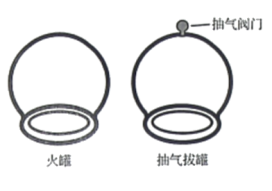
\includegraphics[height = 3.0cm]{/Users/mac/Desktop/ALLDATA/程序/TEX/实验一/图片4}\label{fig:figure2}
\end{figure}
解:
设火罐体积$V_{10}$,抽气拔罐体积$V_{20}$,由克拉伯龙方程得:
\[\frac{p_{0}V_{10}}{T_{1}} = \frac{p_{1}V_{11}}{T_{0}}\]
即:
\[p_{1} = \frac{7}{10}p_{0}\]
由题可知二者最终状态压强相等,
又抽气拔罐可看作一部分气体发生等温变化且同一压强下同一温度气体体积比等于质量比,则:
\begin{gather*}
    p_{0}V_{21} = \frac{20}{21}p_{1}V_{20}\\
    \frac{m_{2}}{m_{0}} = \frac{V_{20} - V_{21}}{V_{20}}\\
\end{gather*}
整理得:
\begin{gather*}
    p_{1} = \frac{7}{10}p_{0}\\
    \frac{m_{2}}{m_{0}} = \frac{1}{3}\\
\end{gather*}
\paragraph{}


\paragraph{}
    5.(2021高考)某双层玻璃保温杯夹层中有少量空气,温度为$27\,^{\circ}\mathrm{C}$时,压强为$3 \times 10^{3}Pa$。

    (1)当夹层中空气的温度升至$37\,^{\circ}\mathrm{C}$,求此时夹层中空气的压强

    (2)当保温杯外层出现裂隙,静置足够长时间,求夹层中增加的空气质量与原有空气质量的比值,设环境温度为$27\,^{\circ}\mathrm{C}$,大气压强为$1 \times 10^{5}Pa$。

解:
(1) $T_{1} = 300K, T_{2} = 310K$可知气体发生等容变化,可列:
\[\frac{p_{1}}{T_{1}} = \frac{p_{2}}{T_{2}}\]
即:
\[p_{2} = \frac{p_{1}T_{2}}{T_{1}} = 3.1 \times 10^{3}Pa\]

(2)设比值为$\lambda$,有:
\begin{gather*}
    p_{1}V_{0} = p_{0}V_{1}\\
    \lambda = \frac{m_{2} - m_{0}}{m_{0}} = \frac{V_{0} - V_{1}}{V_{1}}\\
\end{gather*}
整理得:
\begin{gather*}
    V_{1} = \frac{p_{1}V_{0}}{p_{0}} = 3 \times 10^{-2}V_{0}\\
    \lambda = \frac{97}{3}\\
\end{gather*}


\paragraph{高考中的气缸与液柱}

\paragraph{}
    6.(2021高考)如图,一汽缸中由活塞封闭有一定量的理想气体,中间的隔板将气体分为A、B两部分;
    初始时,A、B的体积均为V,压强均等于大气压$p_{0}$,隔板上装有压力传感器和控制装置,当隔板两边压强差超过0.5$p_{0}$时隔板就会滑动,否则隔板停止运动。
    气体温度始终保持不变。向右缓慢推动活塞,使B的体积减小为$\frac{V}{2}$。

    (1)求A的体积和B的压强

    (2)再使活塞向左缓慢回到初始位置,求此时A的体积和B的压强。

\begin{figure}[htbp]
% \centering
\paragraph{} 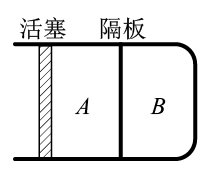
\includegraphics[height = 2.0cm]{/Users/mac/Desktop/ALLDATA/程序/TEX/实验一/图片6}\label{fig:figure3}
\end{figure}

\paragraph{}
\paragraph{}
\paragraph{}
\paragraph{}


\paragraph{}
    7.(2021高考)如图,一玻璃装置放在水平桌面上,竖直玻璃管A、B、C粗细均匀,A、B两管的上端封闭,C管上端开口,三管的下端在同一水平面内且相互连通。
    A、B两管的长度分别为$l_{1}=13.5cm,l_{2}=32cm$。将水银从C管缓慢注入,直至B、C两管内水银柱的高度差h=5cm。
    已知外界大气压为$p_{0}$=75cmHg。
    求A、B两管内水银柱的高度差。

\begin{figure}[htbp]
% \centering
\paragraph{} 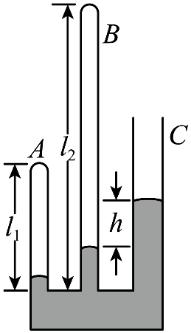
\includegraphics[height = 3.0cm]{/Users/mac/Desktop/ALLDATA/程序/TEX/实验一/图片7}\label{fig:figure4}
\end{figure}




\end{document}